\newcommand{\pageviii}{
\fontsize{10}{11}\selectfont
\heading{Continguts i objectius}

\begin{itemize}
	\item Jerarquia de les operacions.
	\item Nombres decimals i racionals. Transformació de fraccions en decimals i viceversa. Nombres decimals exactes i periòdics. \item Fracció generatriu.
	\item Operacions amb fraccions i decimals. Càlcul aproximat i arrodoniment. Xifres significatives. Error absolut i relatiu.
\end{itemize} 

\begin{itemize}
	\item[1. ] Utilitzar les propietats dels nombres racionals per operar-hi, emprant la forma de càlcul i de notació adequada, per resoldre problemes de la vida quotidiana, i presentant els resultats amb la precisió requerida.
\item[1.1. ] Reconeix els diferents tipus de nombres (naturals, enters, racionals), indica el criteri usat per distingir-los i els fa servir per representar i interpretar adequadament informació quantitativa.
\item[1.2. ] Distingeix, en trobar el decimal equivalent a una fracció, entre decimals finits i decimals infinits periòdics, i en aquest cas indica el grup de decimals que es repeteixen o formen període.
\item[1.6.] Distingeix i empra tècniques adequades per fer aproximacions per defecte i per excés d’un nombre en problemes contextualitzats, i justifica els procediments.
\item[1.10.] Empra nombres racionals per resoldre problemes de la vida quotidiana i analitza la coherència de la solució.
\end{itemize}

}


\newcommand{\pagexxii}{
	\fontsize{10}{11}\selectfont
	\heading{Continguts i objectius}
	
	\begin{itemize}
\item Potències de nombres racionals amb exponent enter. Significat i ús.
\item Potències de base 10. Aplicació per a l’expressió de nombres molt petits. \item Operacions amb nombres expressats en notació científica.
\item Arrels quadrades. Arrels no exactes. Expressió decimal. Expressions radicals: transformació i operacions.

	\end{itemize} 
	
	\begin{itemize}
	\item[1.4. ] Expressa nombres molt grans i molt petits en notació científica, hi opera, amb calculadora i sense, i els empra en problemes contextualitzats.
	\item[1.5. ] Factoritza expressions numèriques senzilles que contenguin arrels, hi opera i simplifica els resultats.

	\end{itemize}
}

\newcommand{\pagexxv}{
\heading{Exemples:}

\begin{example}
	
	\large
	
	\[320\, 000\, 000 =  3,2 \cdot 10^{8} \]
	
	\[0,000\, 00524 =  5,24 \cdot 10^{-6} = 5,24 \text{ micres.} \]
	
	\[475\,000  =  4,75 \cdot 10^{5} \]
	
	\[0,000\,000\,00761  =  7,61 \cdot 10^{-9} \]
\end{example}
}


\newcommand{\pagexxvi}{
	\heading{Operacions en notació científica:}
	
	\begin{theorybox}
		\large
		\begin{itemize}
			\item \textbf{Suma i resta:} 	Expressam tot en la mateixa potència de 10
			
			\[ 2,5\cdot 10^4 + 4,1 \cdot 10^5 - 1,72\cdot 10^3 = \]
			  \[ 25 \cdot 10^3 + 410 \cdot 10^3 - 1,72\cdot 10^3 = 
			   433,28\cdot 10^3 = 4,3328 \cdot 10^5
			\]
			
			\item \textbf{Producte i divisió:} 	Operam els coeficients i les potències per separat 
			
			\[ \frac{4\cdot 10^{12}\cdot 3,5\cdot 10^{-6}}{ 5,2\cdot 10^3 }=
			   \frac{4\cdot 3,5}{ 5,2 } \times \frac{10^{12} \cdot 10^{-6}}{ 10^3}
			 =2,692\cdot 10^{3} \]
		\end{itemize}
	 	 
	 	
	 
	 	
	 	
	\end{theorybox}
}


\newcommand{\pagexxviii}{

	\heading{Pràctica amb la calculadora:}
	
	\begin{blueshaded}
	\large
	Utilitza la calculadora científica per fer les següents operacions:
	
	\begin{tasks}(2)
		\task $3-5\cdot \left[ 2 : \left(3-\frac{3}{2}\right) +5 \right]=$
		
		\task $\frac{1+\sqrt{2}}{1-\sqrt{2}}=$
		
		\task $\sqrt[3]{2,7\cdot 10^4}=$
		
		\task $\sqrt[5]{\pi \cdot 2^{10}}=$
		
		 
	\end{tasks}
\end{blueshaded}
}


\newcommand{\pagexxxiii}{
	
	\heading{Bingo de potències i arrels (1--15):}

\large

 Exemple de construcció d'un cartó de bingo:
 \begin{center}
 	\begin{tabular}{|c|c|c|}
 		\textit{de 1--5} & \textit{de 6--10} & \textit{de 11--15} \\ \hline
 		\textbf{3} & \cellcolor{gray} & \textbf{12}\\ \hline
 		\textbf{5}& \cellcolor{gray} &  \textbf{14}\\ \hline
 		\cellcolor{gray} &\textbf{7} & \textbf{15}\\ \hline
 	\end{tabular}
 \end{center}

\vso
Per a les operacions amb potències compta l'exponent. Les operacions amb arrels compta el resultat:

\Large

\begin{multicols}{2}
	\begin{enumerate} 
		 \setlength{\itemsep}{15pt}
		  \setlength{\labelsep}{10pt}
		\item $\left(a^2\right)^4:a^7$
		\item $\sqrt[4]{16}$
		\item $\frac{\left(a^3\right)^7 \cdot a}{a^{19}}$
		\item $16^{1/2}$
		\item $\sqrt[3]{125}$
		\item $\frac{a^{10} \cdot a^{8}}{a^{12}}$
		\item $\frac{a^6 \cdot a}{a^0}$
		\item $\left(a^3 \cdot a \right)^2$
		\item $\left[\left(a^2 \right)^2\right]^2 \cdot a$
		\item $\sqrt[3]{10^{3}}$
		\item $\frac{ \left(a^4\cdot a^2\right)^2}{a}$
		\item $(a^4)^4:a^4$
		\item $\sqrt{169}$
		\item $\frac{(a^2)^6\cdot a^2}{a^0}$
		\item $\left( a^3 \cdot a^2 \right)^3$
	\end{enumerate}
\end{multicols}
}

\newcommand{\pagexxxiv}{
	\fontsize{10}{11}\selectfont
\heading{Continguts i objectius}

\begin{itemize}	
\item 	Successions numèriques. Successions recurrents 
\item Progressions aritmètiques i geomètriques.
\end{itemize}

\begin{itemize}	
\item[2.] Obtenir i manipular expressions simbòliques que descriguin successions numèriques, i observar regularitats en casos senzills que incloguin patrons recursius.
\item[2.1.] Calcula termes d’una successió numèrica recurrent usant la llei de formació a partir de termes anteriors.
\item[2.2.] Obté una llei de formació o fórmula per al terme general d’una successió senzilla de nombres enters o fraccionaris.
\item[2.3.] Identifica progressions aritmètiques i geomètriques, n’expressa el terme general, calcula la suma dels “n” primers termes, i les empra per resoldre problemes.
\item[2.4.] Valora i identifica la presència recurrent de les successions en la naturalesa i resol problemes associats.
\end{itemize}	
}


\newcommand{\pagexxxviii}{
 \heading{Raona:}
 
 \begin{center}
 	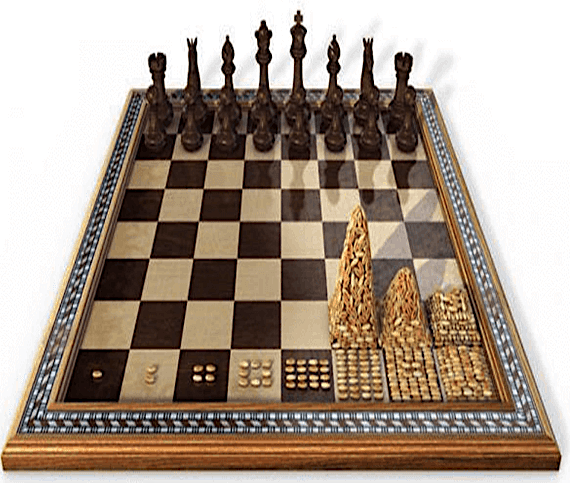
\includegraphics[width=0.44\textwidth]{img-sol/ajedrez} 
 	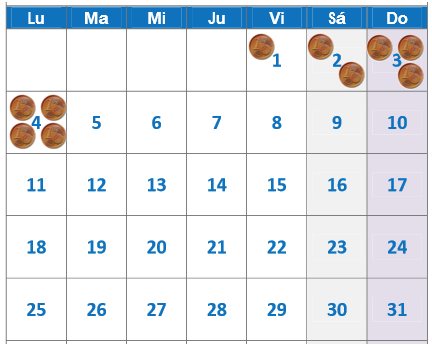
\includegraphics[width=0.44\textwidth]{img-sol/calendario} 
 \end{center}
}

\newcommand{\pagexliii}{
	 \heading{Quina és la fitxa que falta?}
	 
	 \begin{tasks}(2)
	 	\task 	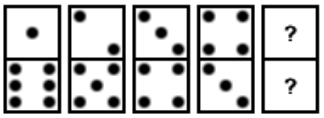
\includegraphics[width=0.4\textwidth]{img-sol/domino-seq-1} 
	 	
	 	\task	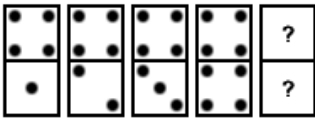
\includegraphics[width=0.4\textwidth]{img-sol/domino-seq-2} 
	 	
	 	\task	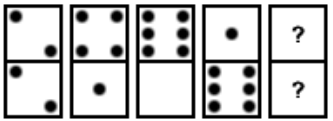
\includegraphics[width=0.4\textwidth]{img-sol/domino-seq-3} 
	 	
	 	\task	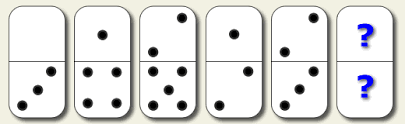
\includegraphics[width=0.4\textwidth]{img-sol/domino-seq-4} 
	 \end{tasks}
 
 \vso
 
  \heading{Quin és el terme general?}
  
  
  
  \begin{tasks} 
 	\task Quina d'aquestes fórmules proporciona el nombre de punts d'aquesta seqüència de figures?
 	
 	
 	\begin{center}
 		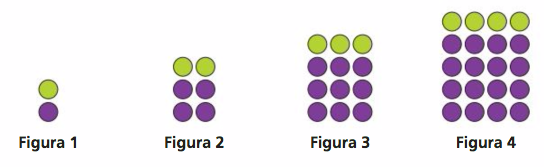
\includegraphics[width=0.5\textwidth]{img-sol/serie-2}
 		
 			a) $n^2+1$ \quad	\qquad b) $n^2+n$	\quad\qquad c) $2n^2$ d)	\quad\qquad $n(n^2+1)$
 	\end{center} 
 
 
 
 	\task  Quants de punts s'utilitzen en l'enèsima figura?
 	
 			\begin{center}
 			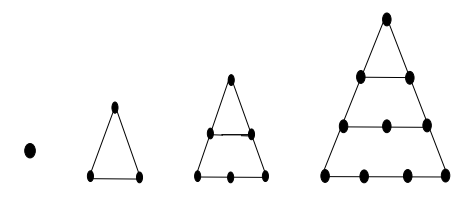
\includegraphics[width=0.5\textwidth]{img-sol/serie-1}
 			\end{center} 
  
 \end{tasks}
}


\newcommand{\pagelii}{

\heading{Simulacions interactives de probabilitat}

\begin{itemize}
	\item Llançament d'una moneda: \url{https://piworld.es/\#!/home/activity/71/0}
	\item Llançament d'un dau: \url{https://piworld.es/\#!/home/activity/94/0}
	\item Ruleta: \url{https://piworld.es/\#!/home/activity/97/0}
	\item Llançament de dos daus: \url{https://piworld.es/\#!/home/activity/98/0}
	\item Laberint de conills: \url{https://piworld.es/\#!/home/activity/95/0}
	\item Dates d'aniversaris: \url{https://piworld.es/\#!/home/activity/99/0}
	\item Caminata del borracho:  \url{https://piworld.es/\#!/home/activity/96/0}
\end{itemize}

}

\newcommand{\pagexlvii}{
	\begin{center}
	
	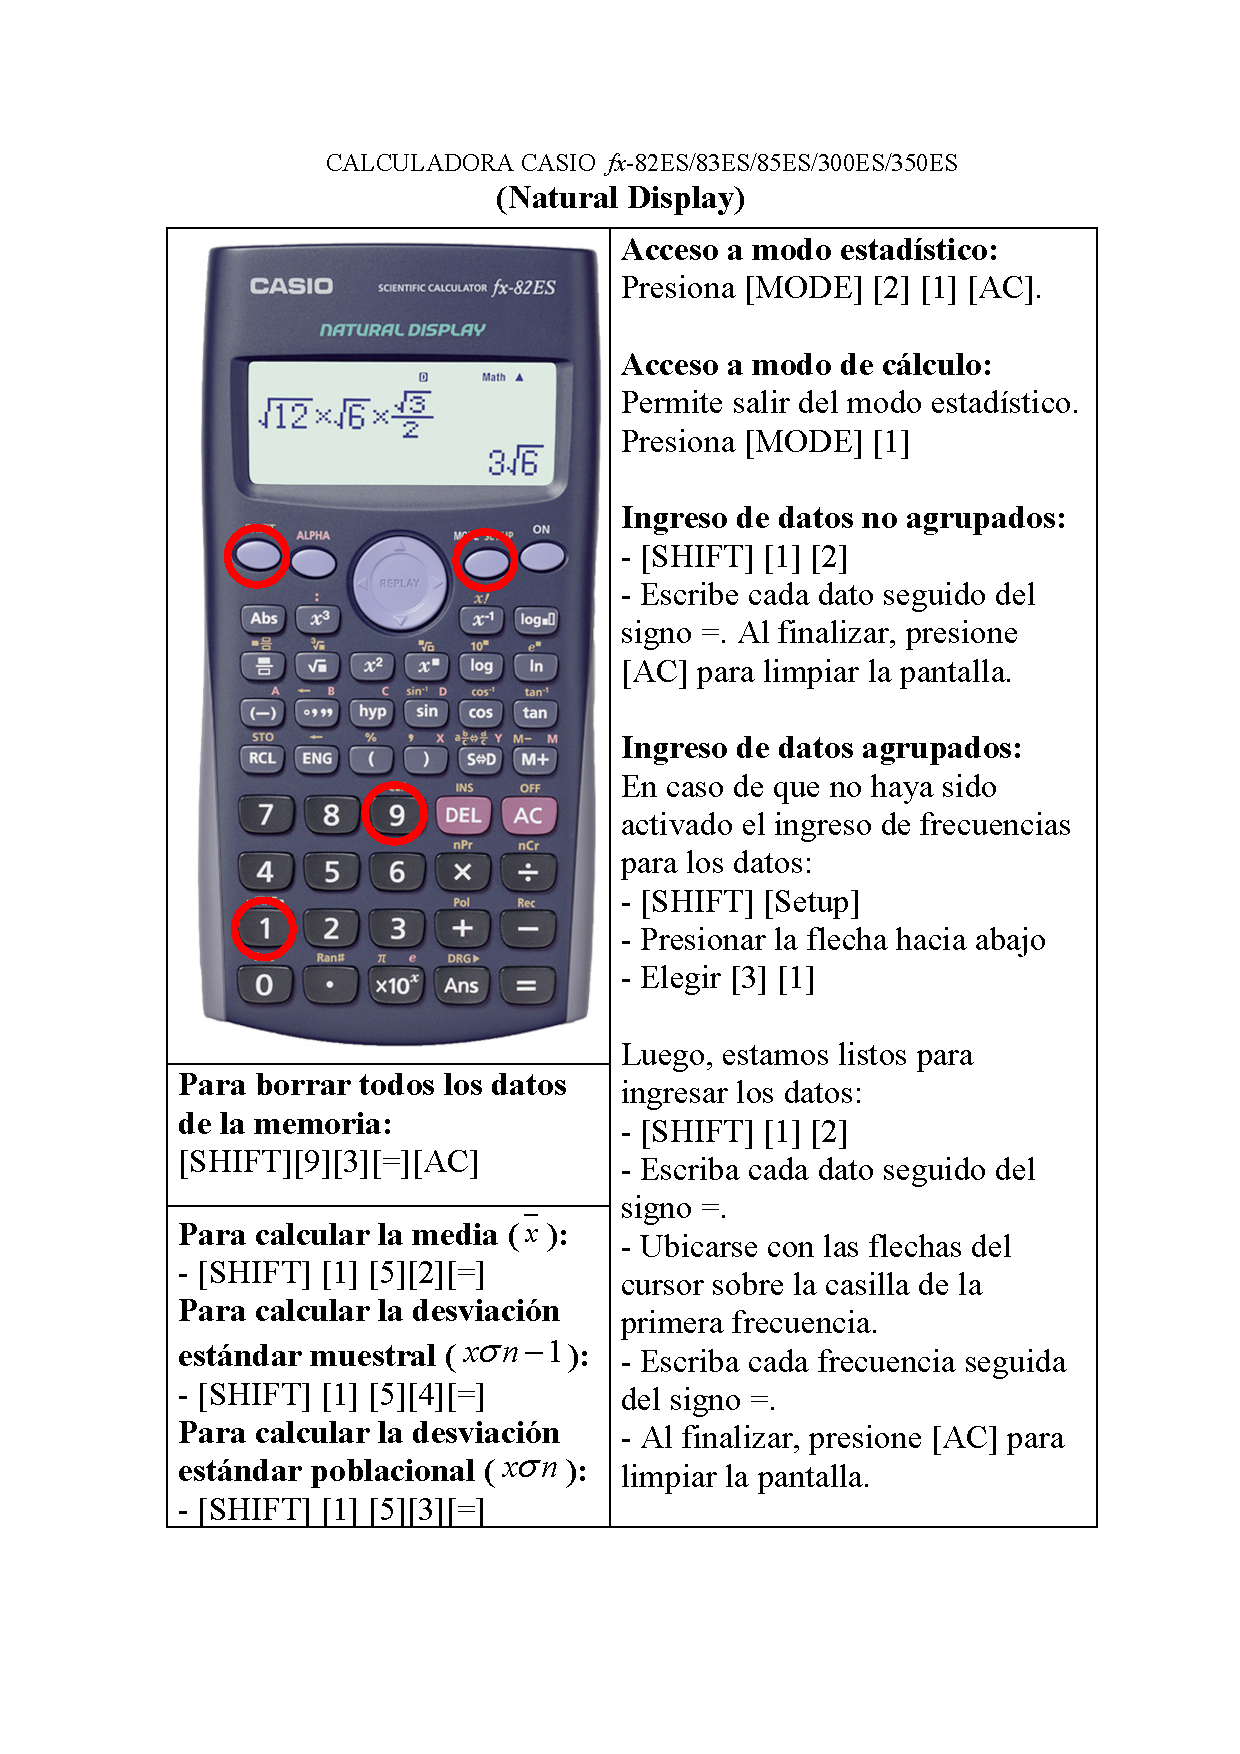
\includegraphics[width=0.85\textwidth]{img-sol/stat-calculadora}
	
	\url{http://beta.upc.edu.pe/matematica/mbcc/paginas/recursos/semana13/CALCULADORAS.doc}
	
	\end{center}
}

\newcommand{\pagelix}{
	\begin{center}
	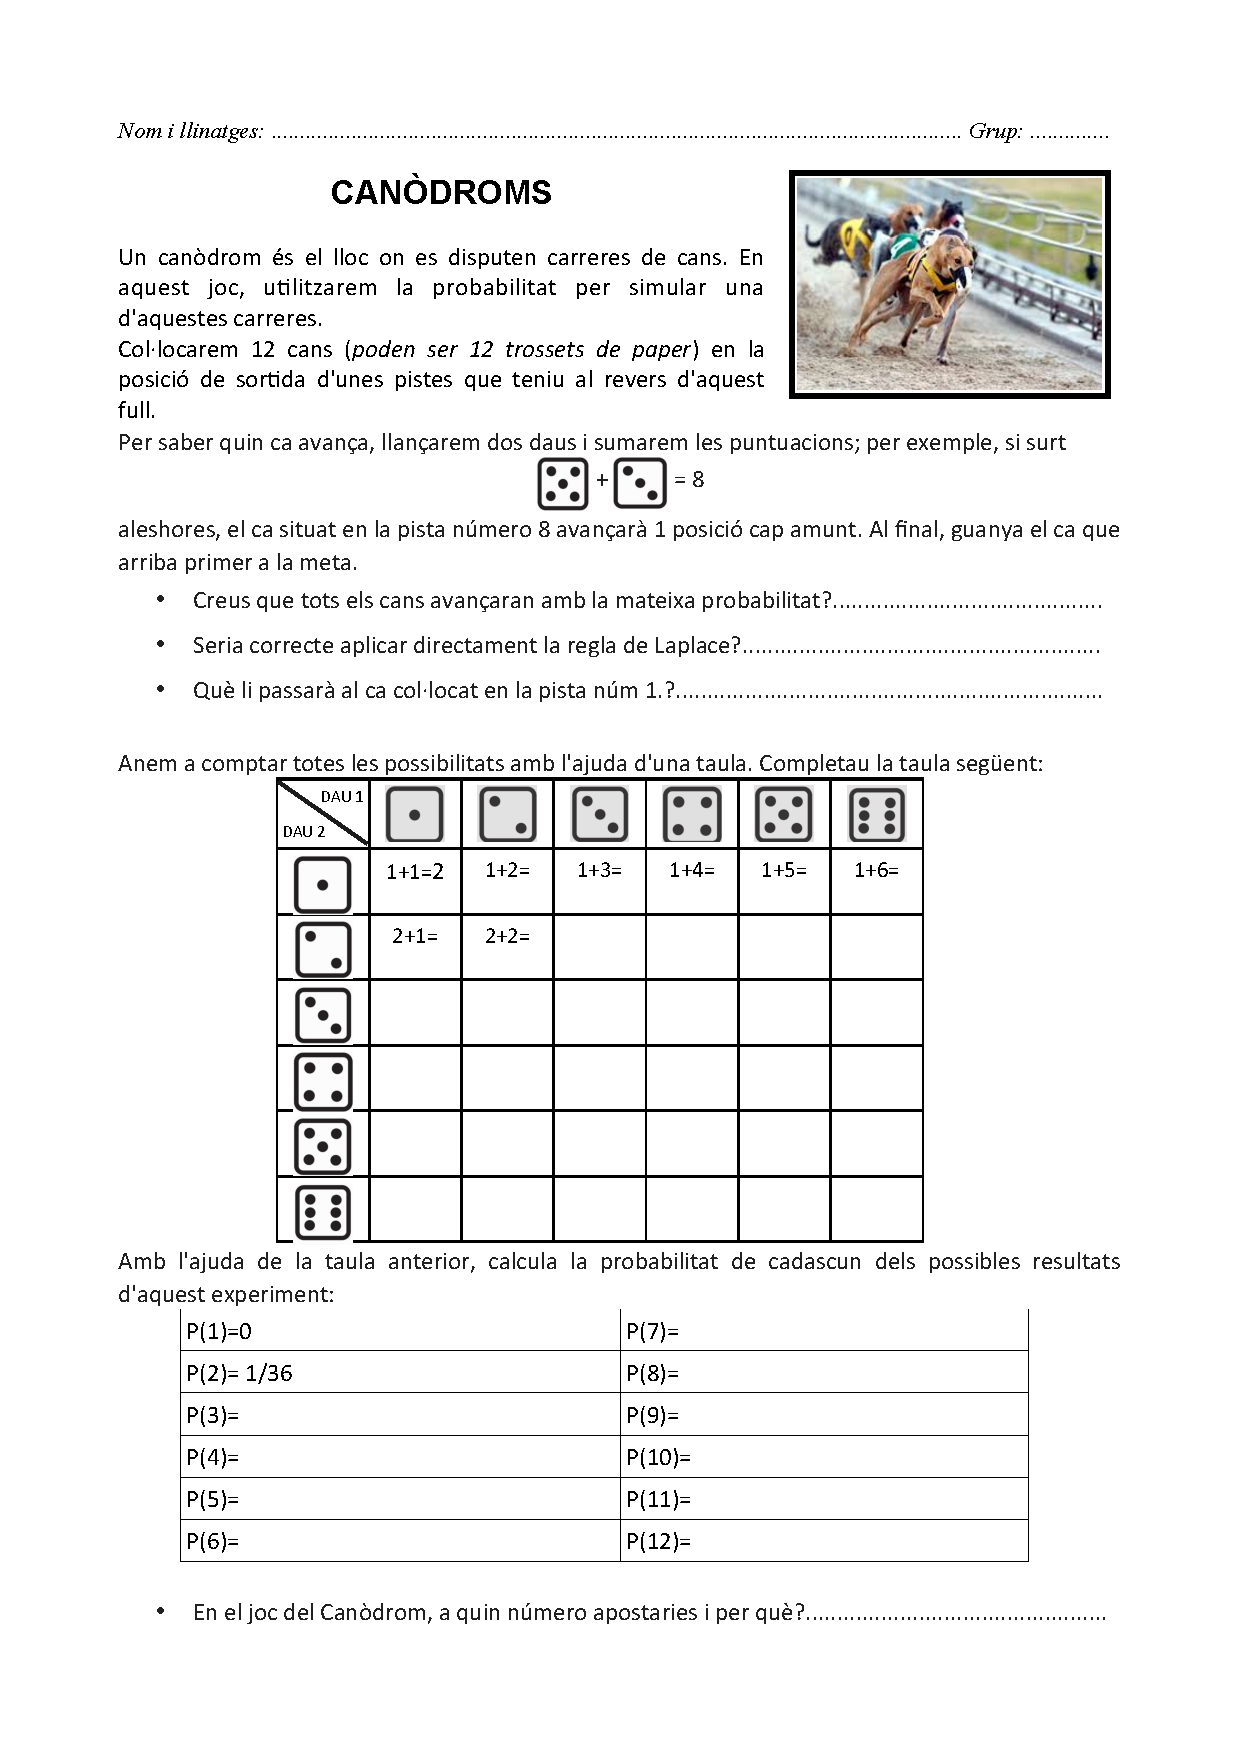
\includegraphics[width=\textwidth]{img-sol/canodromos}
	\end{center}
}


\newcommand{\pagexliv}{
	\fontsize{10}{11}\selectfont
	\heading{Continguts i objectius}
	
	\begin{itemize}	
		\item  Fases i tasques d’un estudi estadístic. Població, mostra. Variables estadístiques: qualitatives, discretes i contínues.
	\item  Mètodes de selecció d’una mostra estadística. Representativitat d’una mostra.
	\item  Freqüències absolutes, relatives i acumulades. Agrupació de dades en intervals.
Gràfics estadístics.
	\item  Paràmetres de posició: mitjana, moda, mediana i quartils. Càlcul, interpretació i propietats.
	\item  Paràmetres de dispersió: rang, recorregut interquartílic i desviació típica. Càlcul i interpretació.
	Diagrama de caixa i bigotis.
	\item Interpretació conjunta de la mitjana i la desviació típica.
	\item Experiències aleatòries. Esdeveniments i espai mostral.
	\item Càlcul de probabilitats mitjançant la regla de Laplace. Diagrames d’arbre senzills. Permutacions, factorial d’un nombre.
	\item Utilització de la probabilitat per prendre decisions fonamentades en diferents contextos.
 	\end{itemize}
	
	\begin{enumerate}	
		\item 
	Elaborar informacions estadístiques per descriure un conjunt de dades mitjançant taules i gràfics adequats a la situació analitzada, i justificar si les conclusions són representatives per a la població estudiada.


\item Calcular i interpretar els paràmetres de posició i de dispersió d’una variable estadística per resumir les dades i comparar distribucions estadístiques.

 \item Analitzar i interpretar la informació estadística que apareix en els mitjans de comunicació, i valorar-ne la representativitat i la fiabilitat.

 \item Estimar la possibilitat que passi un esdeveniment associat a un experiment aleatori senzill, calculant-ne la probabilitat a partir de la freqüència relativa, la regla de Laplace o els diagrames d’arbre, i identificar els elements associats a l’experiment.

	\end{enumerate}	

}

\newcommand{\pagelx}{
	
	\fontsize{10}{11}\selectfont
	\heading{Continguts i objectius}
	
	\begin{itemize}	
	\item Investigació de regularitats, relacions i propietats que apareixen en conjunts de nombres. Expressió usant llenguatge algebraic.
\item Transformació d’expressions algebraiques. Igualtats notables. Operacions elementals amb polinomis.
	\end{itemize}

\begin{enumerate}
	\item[3] Utilitzar el llenguatge algebraic per expressar una propietat o relació donada mitjançant un enunciat, extreure’n la informació rellevant i transformar-la.
\item[3.1.] Fa operacions amb polinomis i els empra en exemples de la vida quotidiana.
\item[3.2.] Coneix i fa servir les identitats notables corresponents al quadrat d’un binomi i una suma per diferència, i les aplica en un context adequat.
\item[3.3.] Factoritza polinomis de grau 4 amb arrels enteres mitjançant l’ús combinat de la regla de Ruffini, identitats notables i extracció del factor comú.
\end{enumerate}

}

\newcommand{\pagelxi}{
	\heading{Dóna una expressió algebraica per a l'àrea pintada }
	
	\vsoo
 
	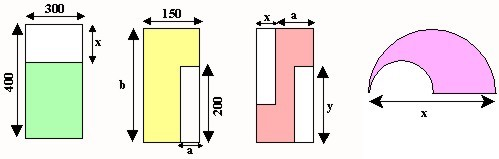
\includegraphics[width=\textwidth]{img-sol/areas-algebra}
 
}

\newcommand{\pagelxii}{

\begin{longtable}{|p{7cm}|p{3cm}|p{3cm}|}\hline
\rowcolor{lightgray} 	\textbf{Frase} & \textbf{Expressió} &  \textbf{Expressió simplificada} \\ \hline
Aina tenia $x$ punts	& $x$ & \\ \hline
Isabel, el doble d'Aina menys 100 punts.	& & \\ \hline
A Pau li faltaven 500 punts per
arribar a Isabel	& & \\ \hline
Sergio va aconseguir el triple d'Aina més 300
punts.	& & \\ \hline
El de Pilar menys el d'Isabel és 3 vegades el
d'Ana. Pilar va tenir llavors:	& & \\ \hline
Marta va tenir la cinquena part del que de Pilar.	& & \\	 \hline	
A Rafael li falten 1000 punts per tenir el
de Sergio.	& & \\	 \hline
Si a Raquel li llevés Ana Belen 500
punts, tindria com Ana. Raquel té:		& & \\	 \hline
Patricia té dues vegades els de Raquel, més
100 punts.			& & \\	 \hline
Juntes, Teresa i Patricia, sumen tres vegades
el d'Ana. Teresa té:				& & \\	 \hline	
Daniel va obtenir la tercera part de Sergio
més 2000 punts.			& & \\		 \hline
\end{longtable}
 
}


\newcommand{\pagelxxv}{
\heading{Solucions dominó d'identitats notables}

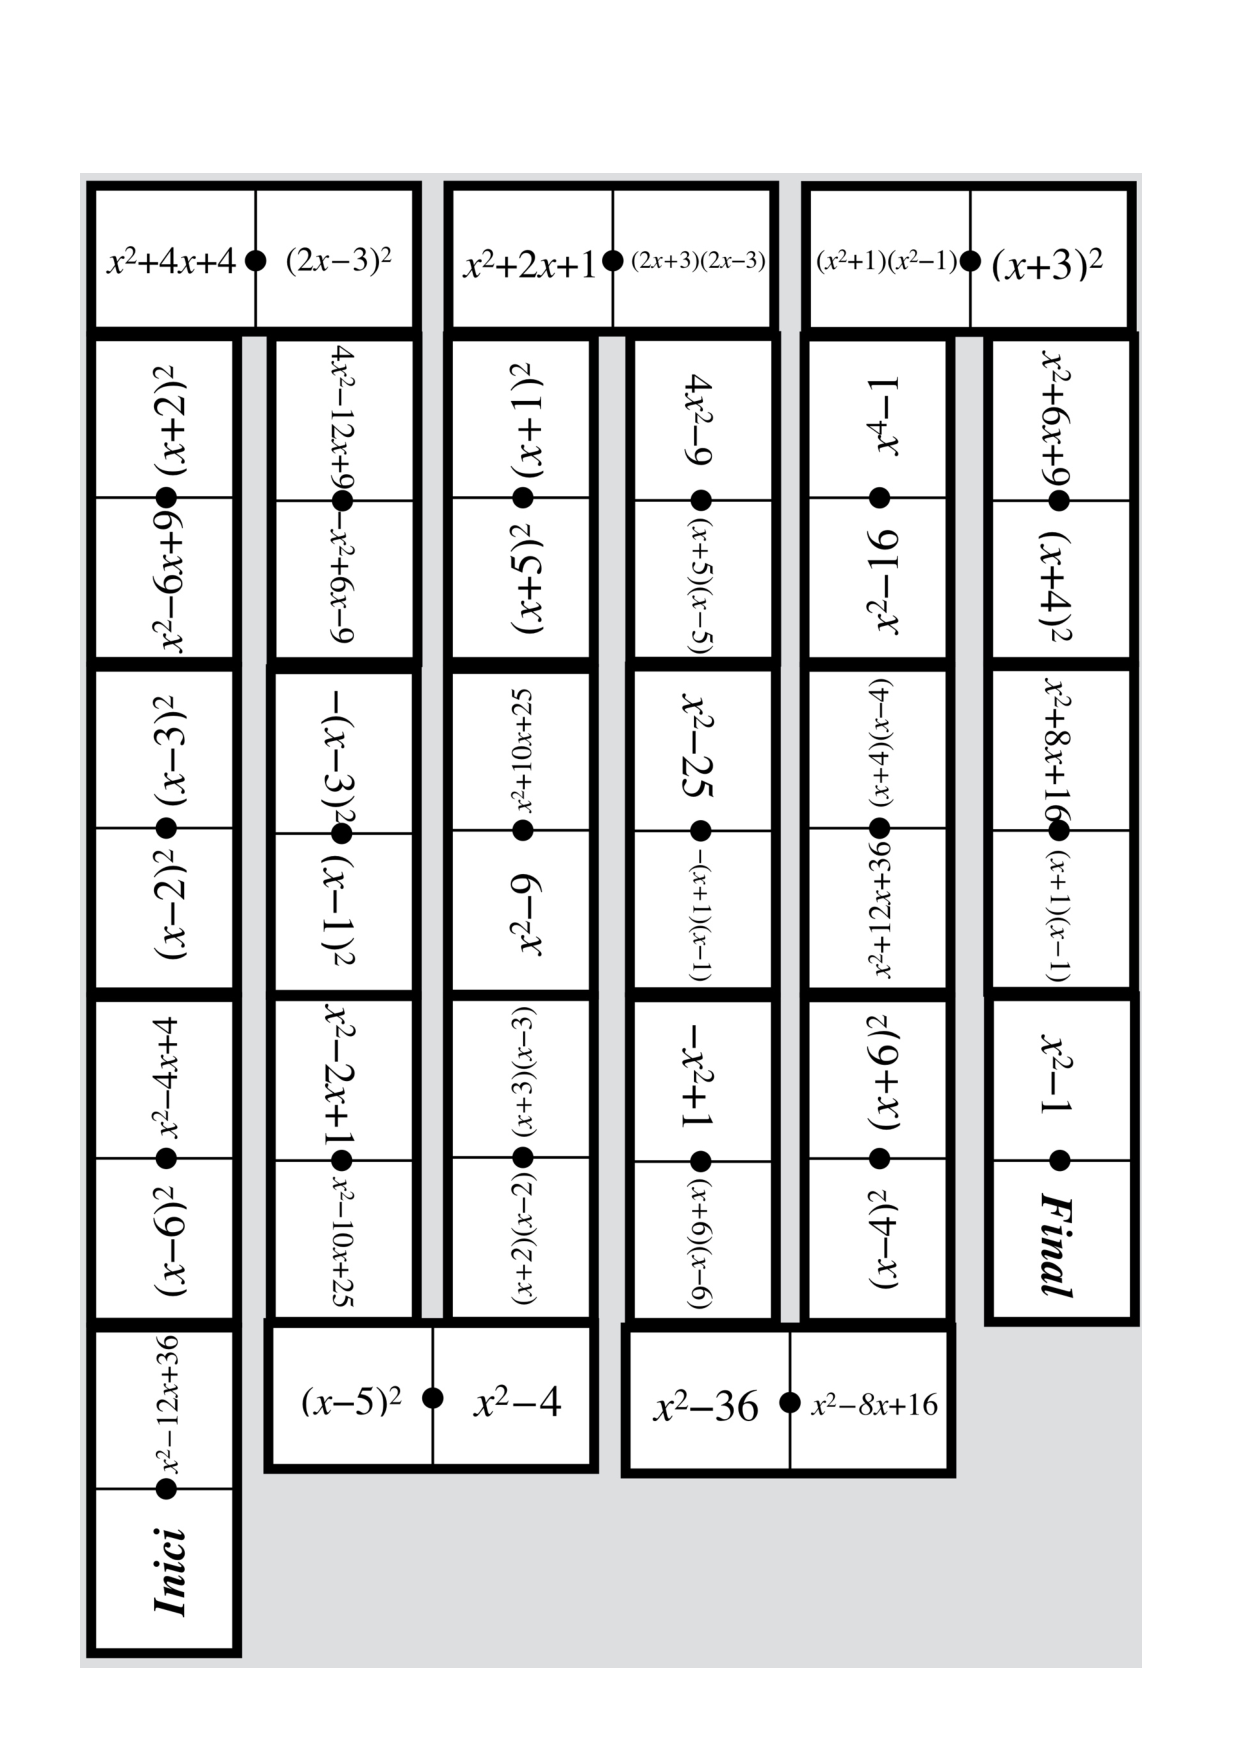
\includegraphics[width=\textwidth]{img-sol/domino-identitats-notables}
}


\newcommand{\pagelxxvi}{
 	
 \fontsize{10}{11}\selectfont
 \heading{Continguts i objectius}
 
 \begin{itemize}	
 	\item Equacions de segon grau amb una incògnita. Resolució (mètode algebraic i gràfic).
\item  Resolució d’equacions senzilles de grau superior a dos.
\item  Resolució de problemes mitjançant la utilització d’equacions i sistemes d’equacions.
 \end{itemize}

\begin{enumerate}
	\item[4.] Resoldre problemes de la vida quotidiana en els quals es necessiti el plantejament i la resolució d’equacions de primer i segon grau, equacions senzilles de grau superior a dos i sistemes de dues equacions lineals amb dues incògnites, aplicant tècniques de manipulació algebraiques, gràfics o recursos tecnològics, i valorar i contrastar els resultats obtinguts.
\item[4.1.] Formula algebraicament una situació de la vida quotidiana mitjançant equacions i sistemes d’equacions, les resol i interpreta críticament el resultat obtingut.
\end{enumerate}
}

\newcommand{\pagelxxvii}{
	\heading{Quantes de micos equivalen a un be?}
	\begin{center}
		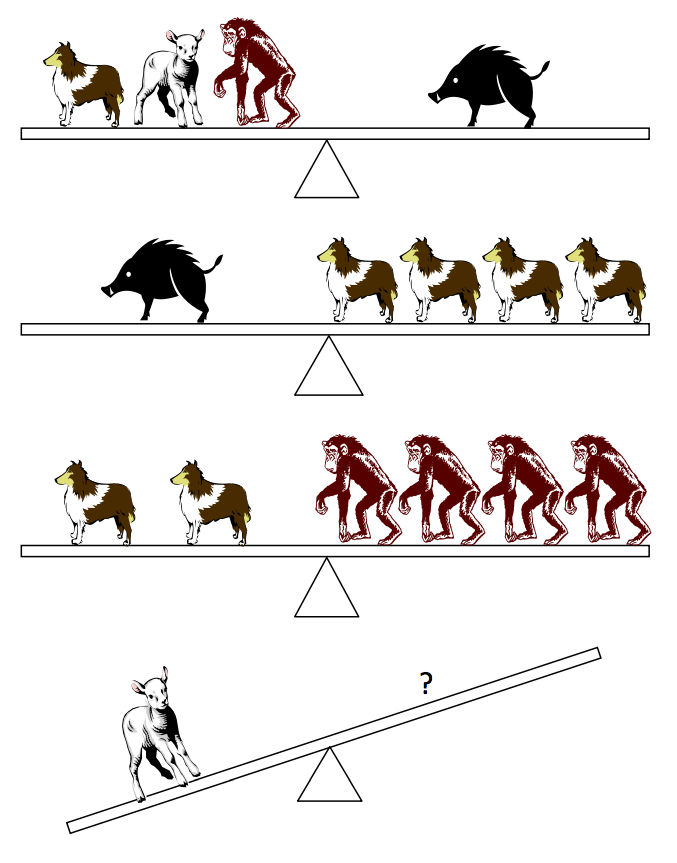
\includegraphics[width=0.5\textwidth]{img-sol/balanza2}
	\end{center}
}

\newcommand{\pagelxxxv}{
	\heading{Què val cada fruita?}
	\begin{center}
		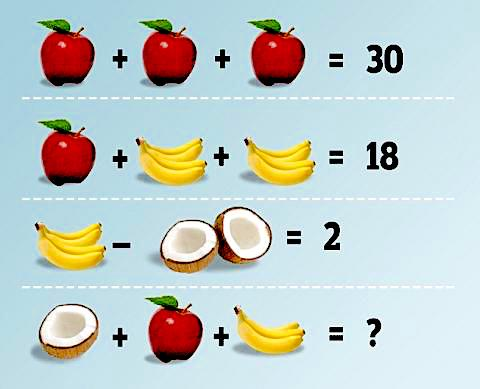
\includegraphics[width=0.6\textwidth]{img-sol/tutifruti}
	\end{center}

\vso
	
	\heading{Quin és el valor de cada animal?}
	\begin{center}
		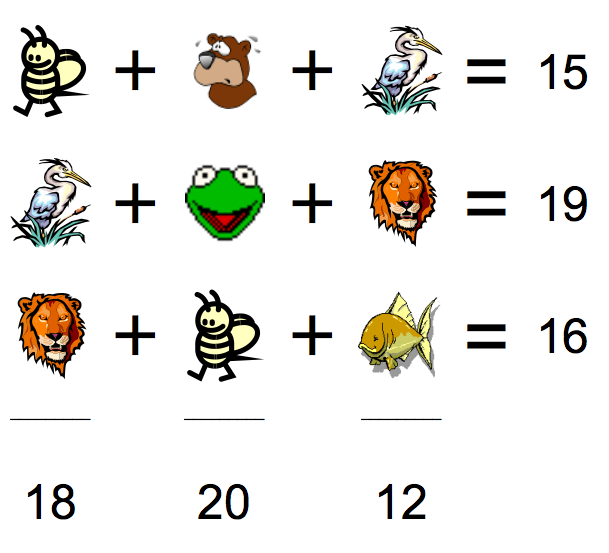
\includegraphics[width=0.6\textwidth]{img-sol/animals}
	\end{center}
}

\newcommand{\pagexci}{
	\heading{Trencaclosques d'equacions:}
	\begin{center}
		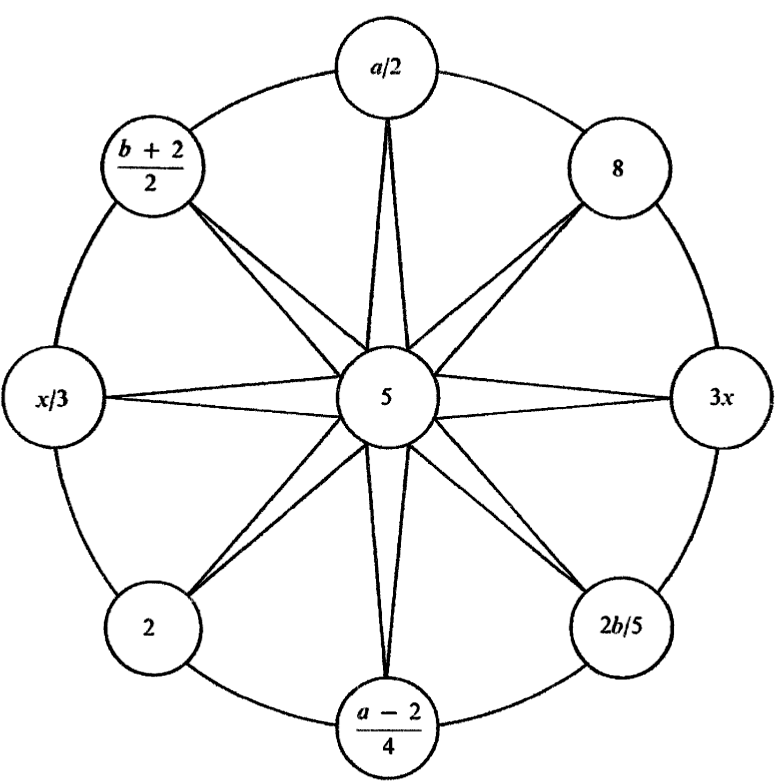
\includegraphics[width=0.6\textwidth]{img-sol/rueda}
	\end{center}

	\Large
	Sabent que els nombres col·locats en un diametre sumen el mateix, troba els valors de $x$, $a$ i $b$.
	
	\begin{center}
		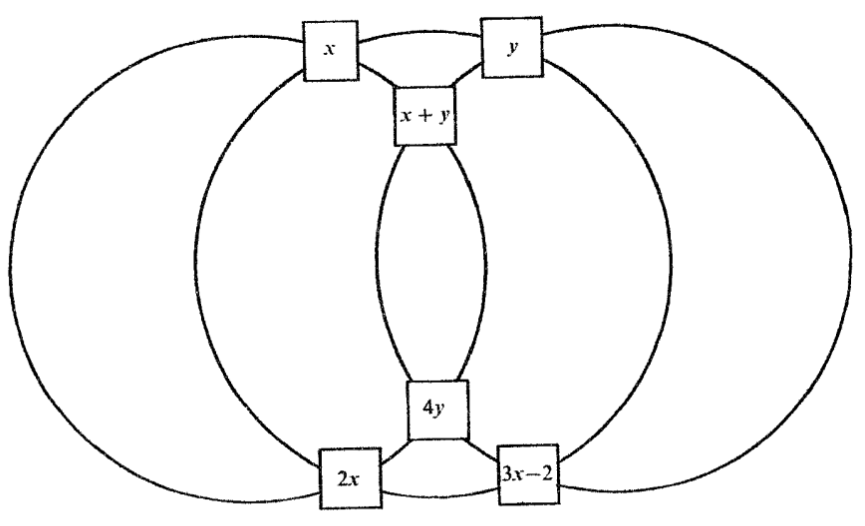
\includegraphics[width=0.9\textwidth]{img-sol/cercles-magics}
	\end{center}
	
	Sabent que els nombres damunt qualsevol circumferència sumen 30, troba els valors de $x$ i $y$.
	
}

\newcommand{\pagecii}{
	\fontsize{10}{11}\selectfont
	\heading{Continguts i objectius}
	
	\begin{itemize}	
		\item    Anàlisi i descripció qualitativa de gràfiques que representen fenòmens de l’entorn quotidià i d’altres matèries.
\item    Anàlisi d’una situació a partir de l’estudi de les característiques locals i globals de la gràfica corresponent.
\item    Anàlisi i comparació de situacions de dependència funcional donades mitjançant taules i enunciats.
\item    Ús de models lineals per estudiar situacions provinents dels diferents àmbits de coneixement i de la vida quotidiana, mitjançant la confecció de la taula, la representació gràfica i l’obtenció de l’expressió algebraica.
\item    Expressions de l’equació de la recta.
\item    Funcions quadràtiques. Representació gràfica. Utilització per representar situacions de la vida quotidiana.
	\end{itemize}

\begin{enumerate}
	\item[1.] Conèixer els elements que intervenen en l’estudi de les funcions i la seva representació gràfica.
\item[1.1.] Interpreta el comportament d’una funció donada gràficament i associa 
enunciats de problemes contextualitzats a gràfiques.
\item[1.2.] Identifica les característiques més rellevants d’una gràfica i les interpreta dins el seu context.
\item[1.3.] Construeix una gràfica a partir d’un enunciat contextualitzat i descriu el fenomen exposat.
\item[1.4.] Associa raonadament expressions analítiques a funcions donades gràficament.
\item[2.] Identificar relacions de la vida quotidiana i d’altres matèries que es poden modelitzar mitjançant una funció lineal i valorar la utilitat de la descripció d’aquest model i dels seus paràmetres per descriure el fenomen analitzat.
\item[2.1.] Determina les diferents formes d’expressió de l’equació de la recta a partir d’una de donada (equació punt-pendent, general, explícita i per dos punts), n’identifica punts de tall i pendent, i la representa gràficament.
\item[2.2.] Obté l’expressió analítica de la funció lineal associada a un enunciat i la representa.
\item[2.3.] Formula conjectures sobre el comportament del fenomen que representa una gràfica i la seva expressió algebraica.
\item[3.] Reconèixer situacions de relació funcional que necessiten ser descrites mitjançant funcions quadràtiques i calcular-ne els paràmetres i les característiques.
\item[3.1.] Calcula els elements característics d’una funció polinòmica de grau dos i la representa gràficament.
\item[3.2.] Identifica i descriu situacions de la vida quotidiana que puguin ser modelitzades mitjançant funcions quadràtiques, les estudia i les representa amb mitjans tecnològics quan sigui necessari.
\end{enumerate}
 
}


\newcommand{\pagecxxvii}{

\heading{Àrees per triangulació}
	\begin{center}
		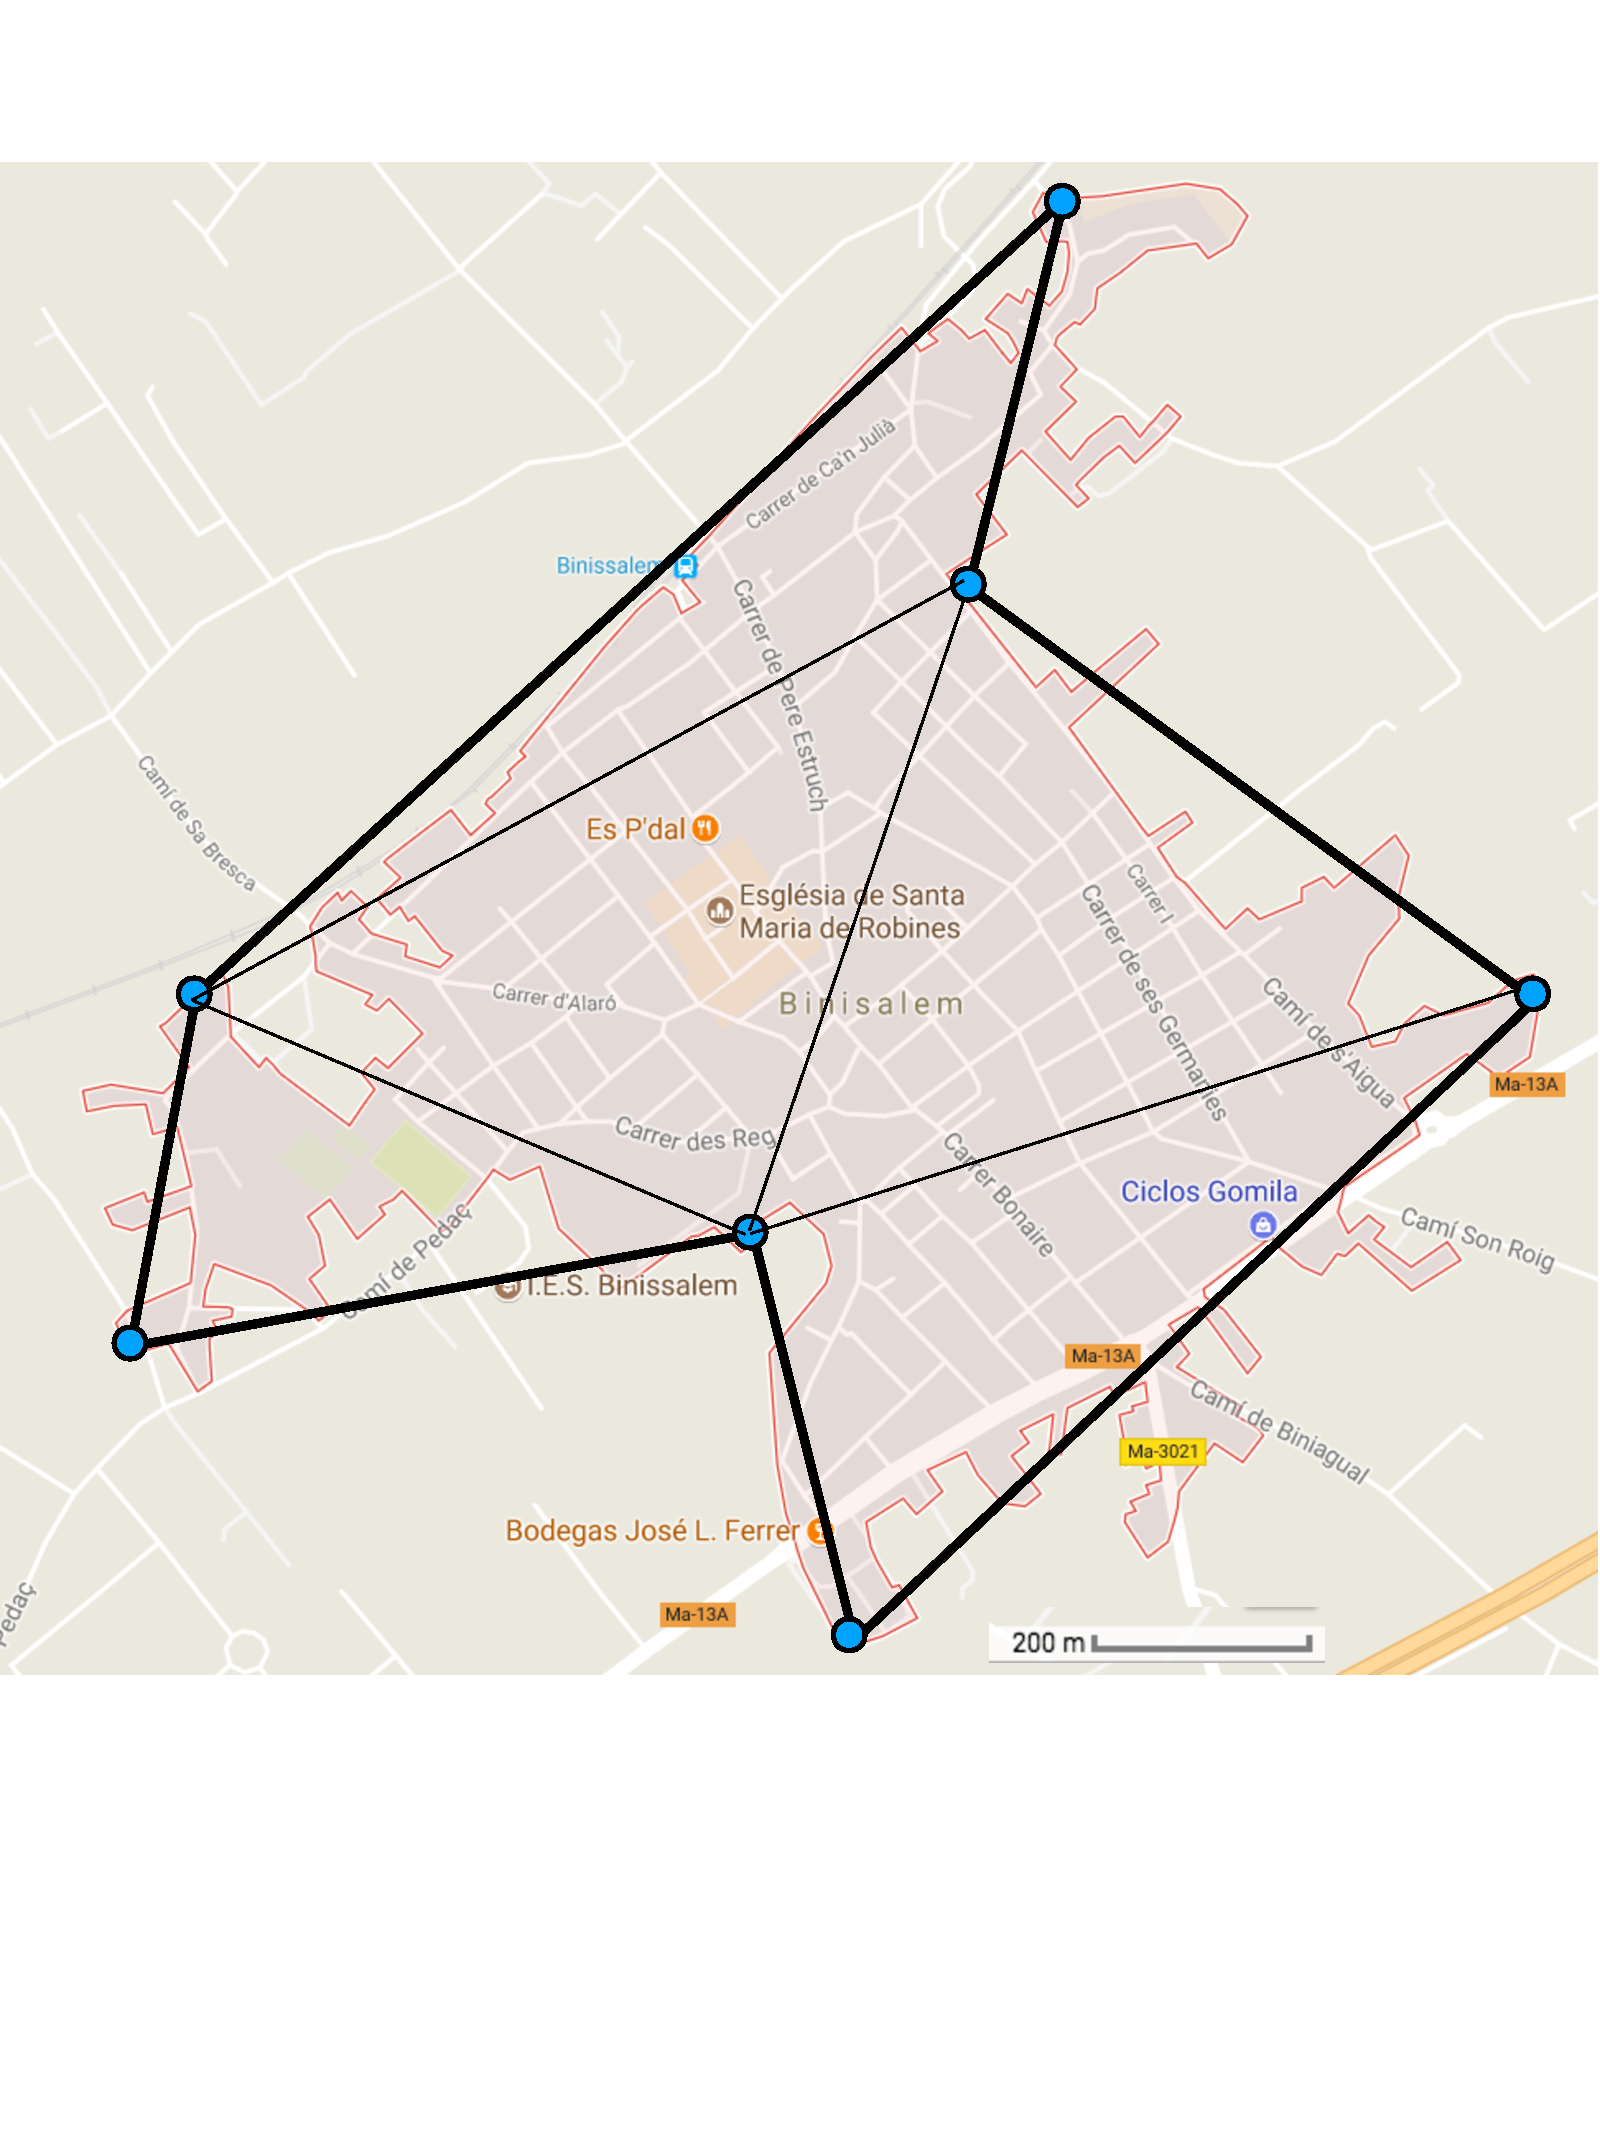
\includegraphics[width=0.8\textwidth]{img-sol/triangulacio}
		
		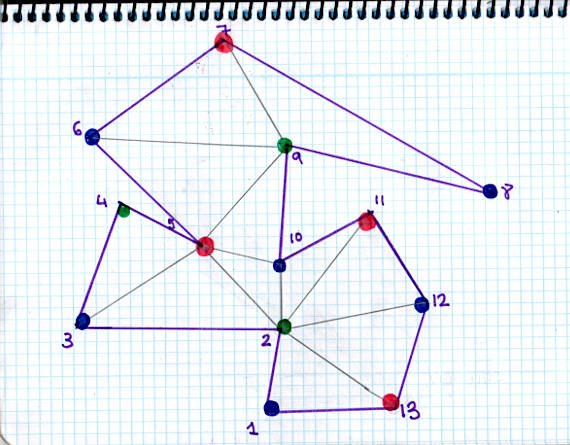
\includegraphics[width=0.8\textwidth]{img-sol/triangulacio2}
		
	\end{center}
}

\newcommand{\pagecxxxix}{
\heading{Què tenen en comú aquestes imatges?}
\begin{center}
	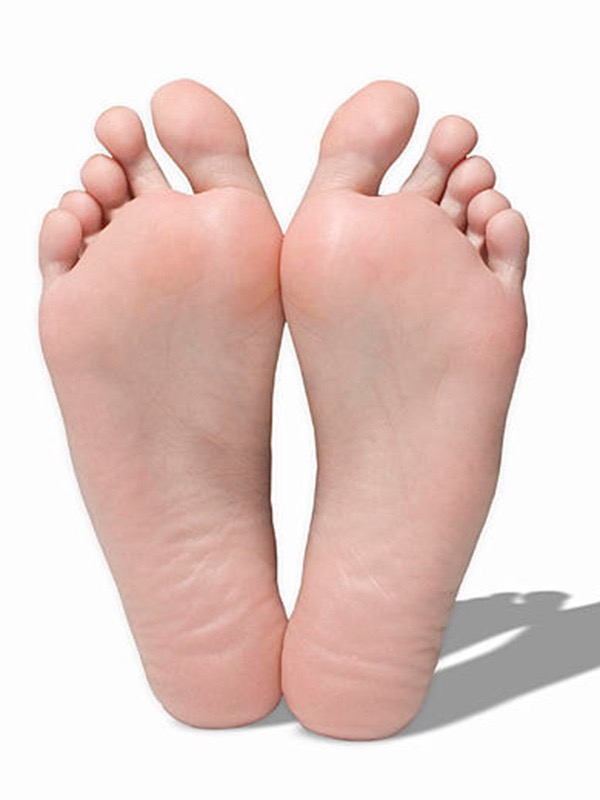
\includegraphics[width=0.4\textwidth]{img-sol/peus}
	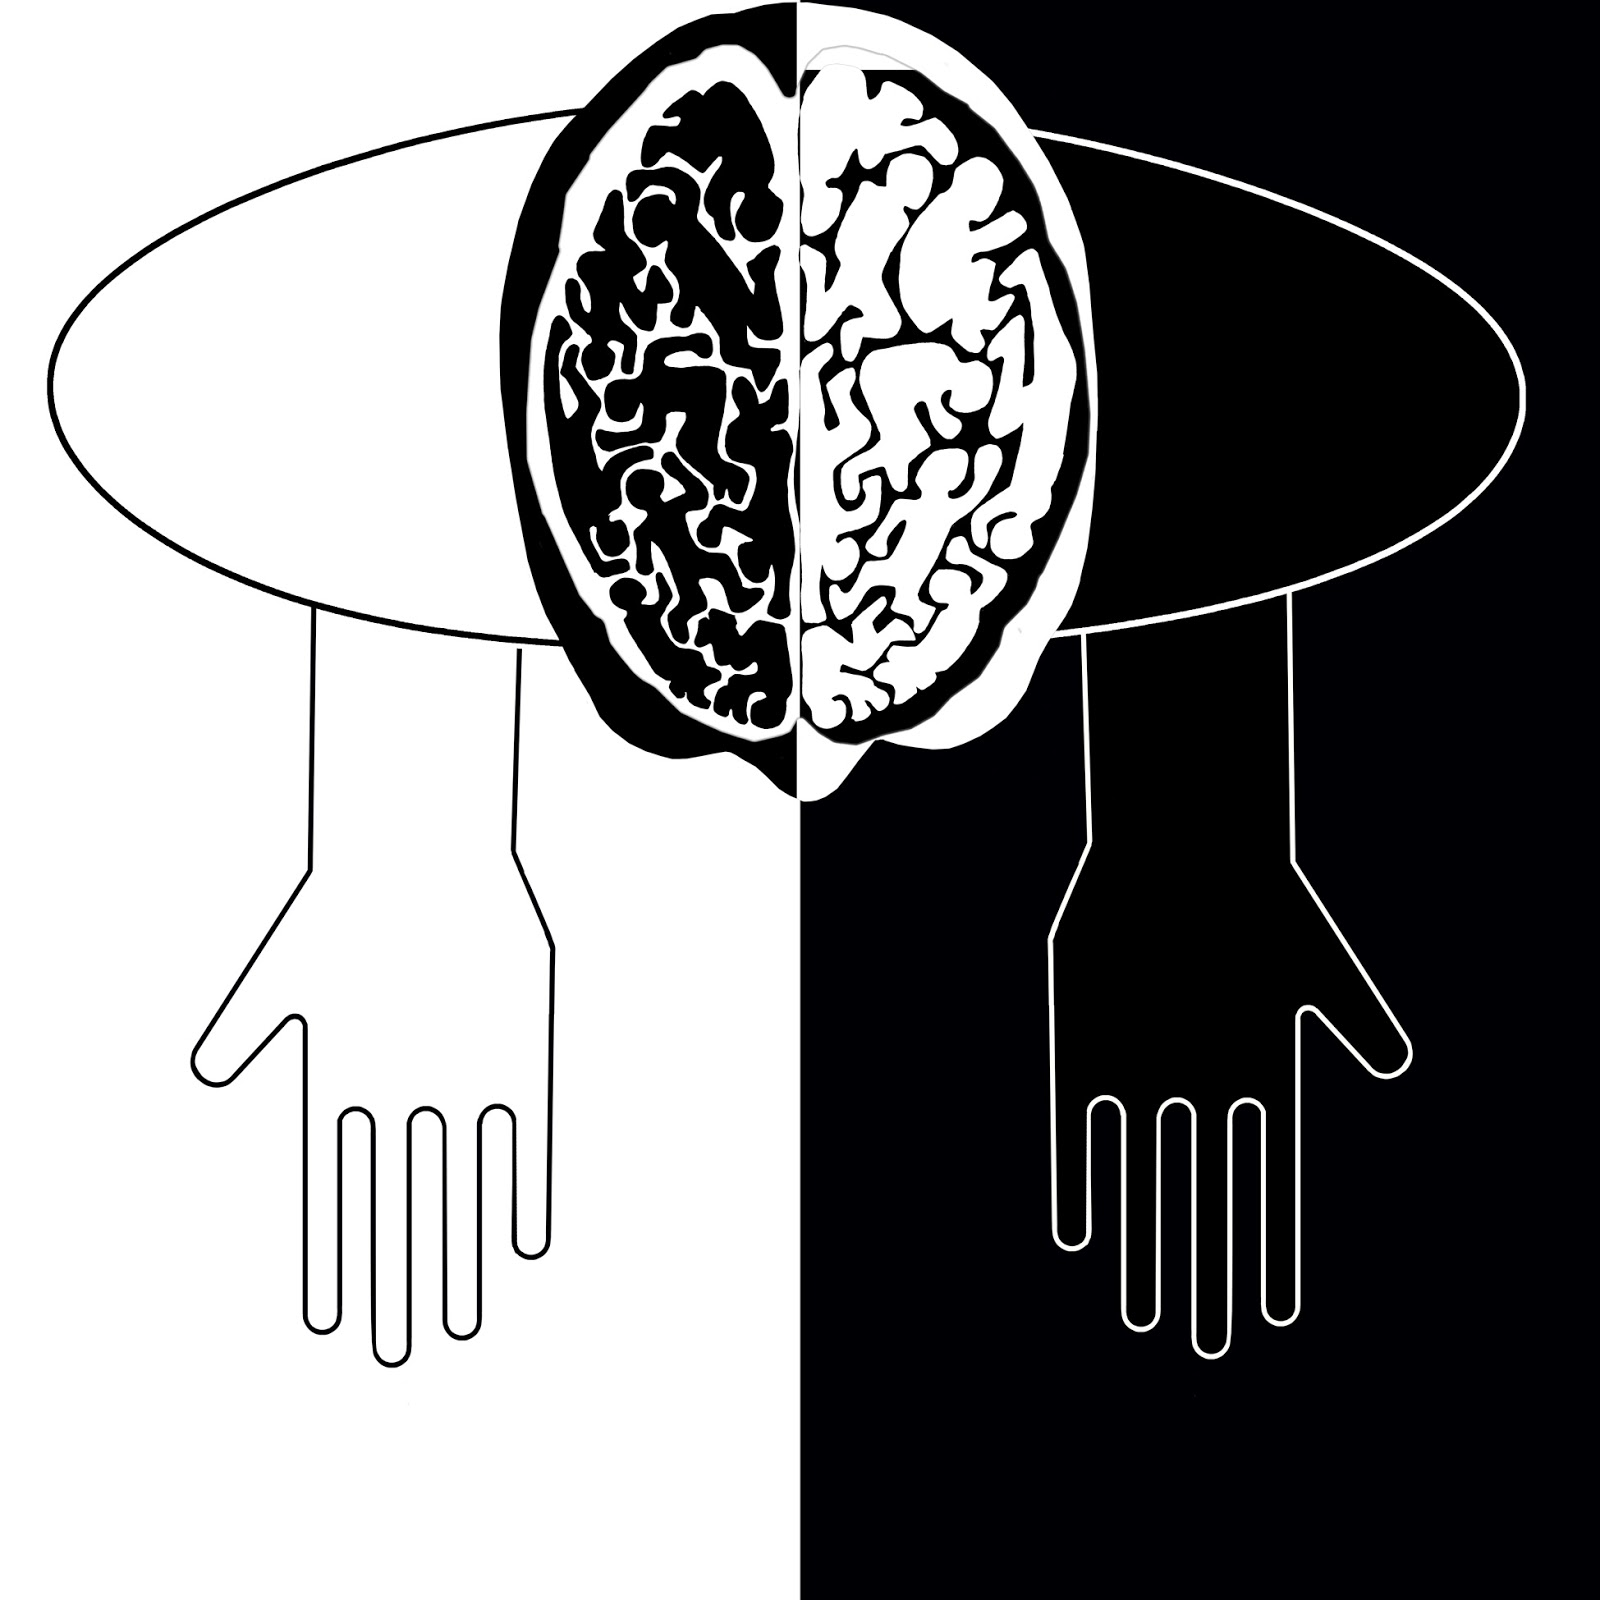
\includegraphics[width=0.4\textwidth]{img-sol/mans}
	
	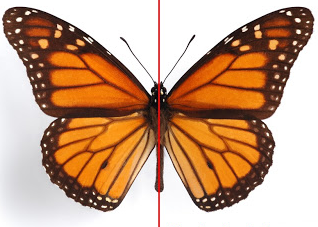
\includegraphics[width=0.4\textwidth]{img-sol/mariposa}
	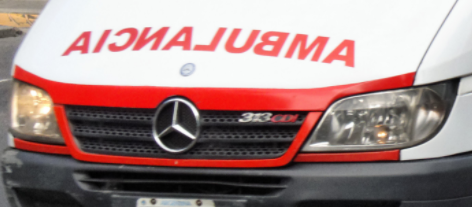
\includegraphics[width=0.4\textwidth]{img-sol/ambulancia}
	
\end{center}
}



\newcommand{\pagecxiv}{
	\fontsize{10}{11}\selectfont
\heading{Continguts i objectius}

\begin{itemize}	
	\item    Geometria del pla.
Mediatriu, bisectriu, angles. Relacions, perímetre i àrea. Propietats.
Lloc geomètric.
Teorema de Tales. Divisió d’un segment en parts proporcionals a altres. Aplicació a la resolució de problemes.

\end{itemize}

\begin{enumerate}
	\item[1.] Reconèixer i descriure els elements i les propietats característiques de les figures planes, els cossos geomètrics elementals i les seves configuracions geomètriques.
\item[1.1.]  Coneix les propietats dels punts de la mediatriu d’un segment i de la bisectriu d’un angle, i les empra per resoldre problemes geomètrics senzills.
\item[1.2.]  Tracta les relacions entre angles definits per rectes que es tallen o per paral·leles tallades per una secant i resol problemes geomètrics senzills.
\item[1.3.]  Calcula el perímetre i l’àrea de polígons i de figures circulars en problemes contextualitzats aplicant fórmules i tècniques adequades.
\item[2.]  Utilitzar el teorema de Tales i les fórmules usuals per fer mesures indirectes d’elements inaccessibles i per obtenir les mesures de longituds, àrees i volums dels cossos elementals, d’exemples presos de la vida real, de representacions artístiques com pintura o arquitectura o de la resolució de problemes geomètrics.
\item[2.1.]  Divideix un segment en parts proporcionals a altres donats i estableix relacions de proporcionalitat entre els elements homòlegs de dos polígons semblants.
\item[2.2.]  Reconeix triangles semblants i, en situacions de semblança, empra el teorema de Tales per al càlcul indirecte de longituds en contextos diversos.
\item[3.]  Calcular (ampliació o reducció) les dimensions reals de figures donades en mapes o plans, coneixent-ne l’escala.
\item[3.1.]  Calcula dimensions reals de mesures de longituds i de superfícies en situacions de semblança: plans, mapes, fotos aèries.
\end{enumerate}
}


\newcommand{\pagecxxviii}{
	\fontsize{10}{11}\selectfont
	\heading{Continguts i objectius}
	
	\begin{itemize}	
		\item  Translacions, girs i simetries en el pla.	
	\end{itemize}

\begin{enumerate}
	\item[4.] Reconèixer les transformacions que duen d’una figura a una altra mitjançant moviments en el pla, aplicar aquests moviments i analitzar dissenys quotidians, obres d’art i configuracions presents en la naturalesa.
\item[4.1.] Identifica els elements més característics dels moviments en el pla presents en la naturalesa, en dissenys quotidians o en obres d’art.
\item[4.2.] Genera creacions pròpies mitjançant la composició de moviments, emprant eines tecnològiques quan sigui necessari.

\end{enumerate}
}


\newcommand{\pagecxl}{
	\fontsize{10}{11}\selectfont
	\heading{Continguts i objectius}
	
	\begin{itemize}	
		\item   Geometria de l’espai. Àrees i volums. Plans de simetria en els políedres.
\item  L’esfera. Interseccions de plans i esferes.
\item  El globus terraqüi. Coordenades geogràfiques i fusos horaris. Longitud i latitud d’un punt.
\item  Ús d’eines tecnològiques per estudiar formes, configuracions i relacions geomètriques.	
	\end{itemize}
	
	\begin{enumerate}
	\item[5.] Identificar centres, eixos i plans de simetria de figures planes i políedres.
\item[5.1.] Identifica els principals políedres i cossos de revolució, i utilitza el llenguatge amb propietat per referir-se als elements principals.
\item[5.2.] Calcula àrees i volums de políedres, cilindres, cons i esferes, i els aplica per resoldre problemes contextualitzats.
\item[5.3.] Identifica centres, eixos i plans de simetria en figures planes o políedres i en la naturalesa, en l’art i en construccions humanes.
\item[6.] Interpretar el sentit de les coordenades geogràfiques i com s’apliquen en la localització de punts.
\item[6.1.] Situa sobre el globus terraqüi equador, pols, meridians i paral·lels, i és capaç d’ubicar un punt sobre el globus terraqüi coneixent-ne la longitud i la latitud.
		
	\end{enumerate}
}


\newcommand{\pageclv}{
	
	\heading{Esquema}
	\begin{center}
		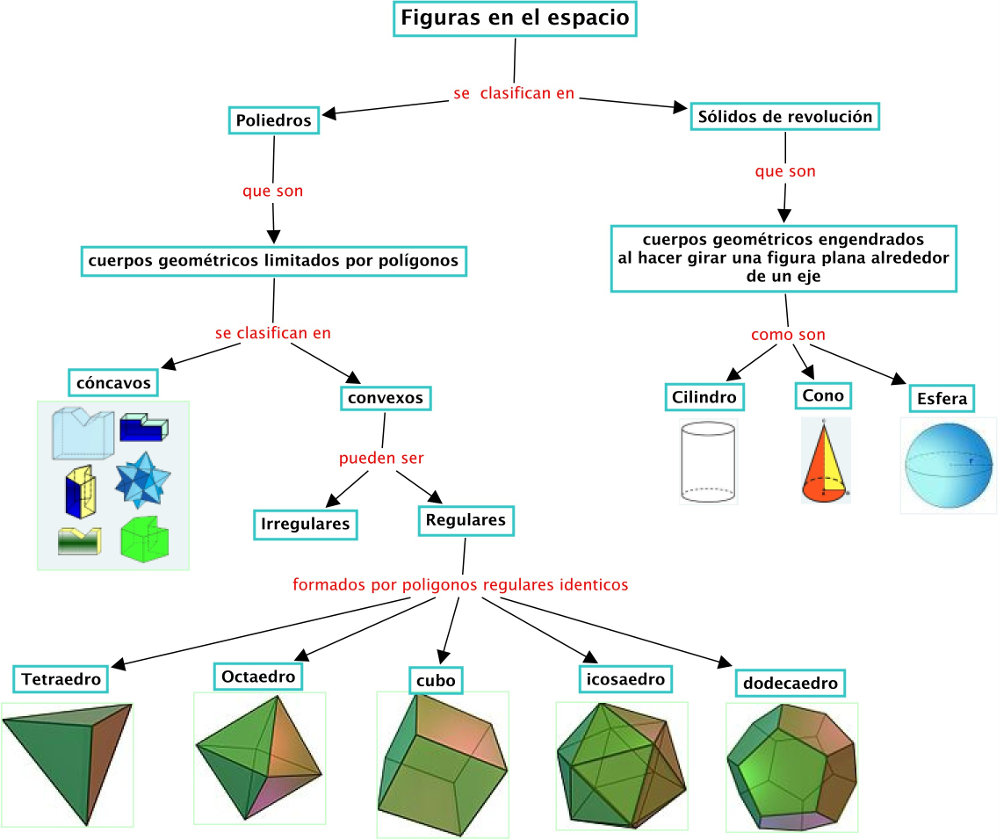
\includegraphics[width=\textwidth]{img-sol/esquema-espacio}
		 
	\end{center}
}

\newcommand{\pagecxli}{
\begin{center}
	
		\begin{center}
		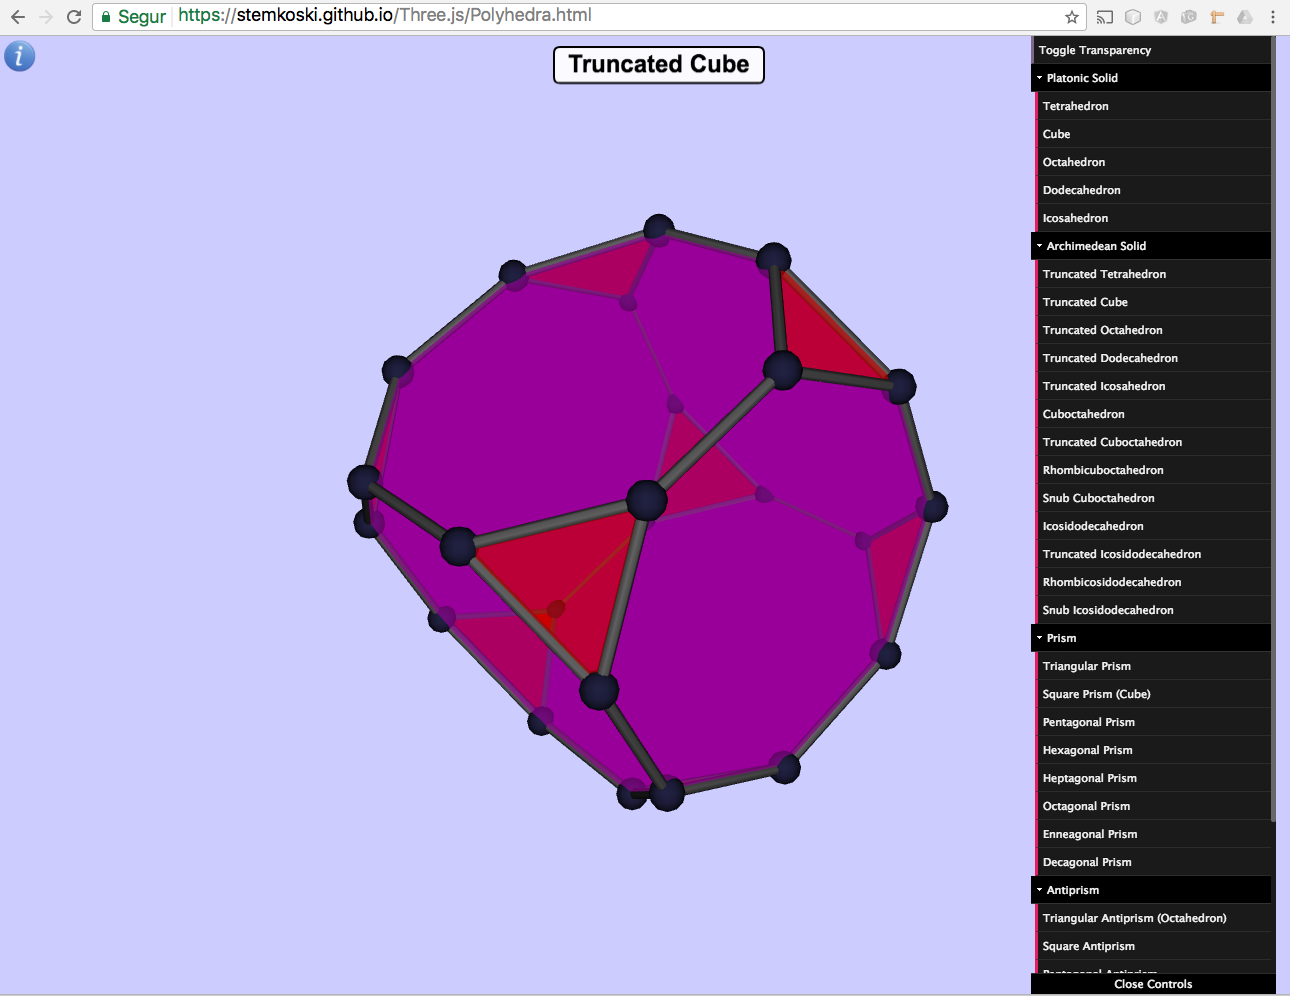
\includegraphics[width=0.6\textwidth]{img-sol/polyedra}
		
	\end{center}
	\href{https://stemkoski.github.io/Three.js/Polyhedra.html}{\textit{Visualització de poliedres 3D:} https://stemkoski.github.io/Three.js/Polyhedra.html}
	

\end{center}
}